\section{Evaluation}
To evaluate the impact flat combining has on the global data structures, we ran a series of experiments to test the raw performance of the data structures themselves under different workloads, and further measured their impact on performance of two simple graph benchmarks.

\subsection{Data Structure Throughput}
First we measured the performance of the global data structures on extremely simple workloads to understand their raw performance.

\begin{figure*}[t]
  \centering
  \begin{subfigure}[b]{0.45\textwidth}
  \centering
  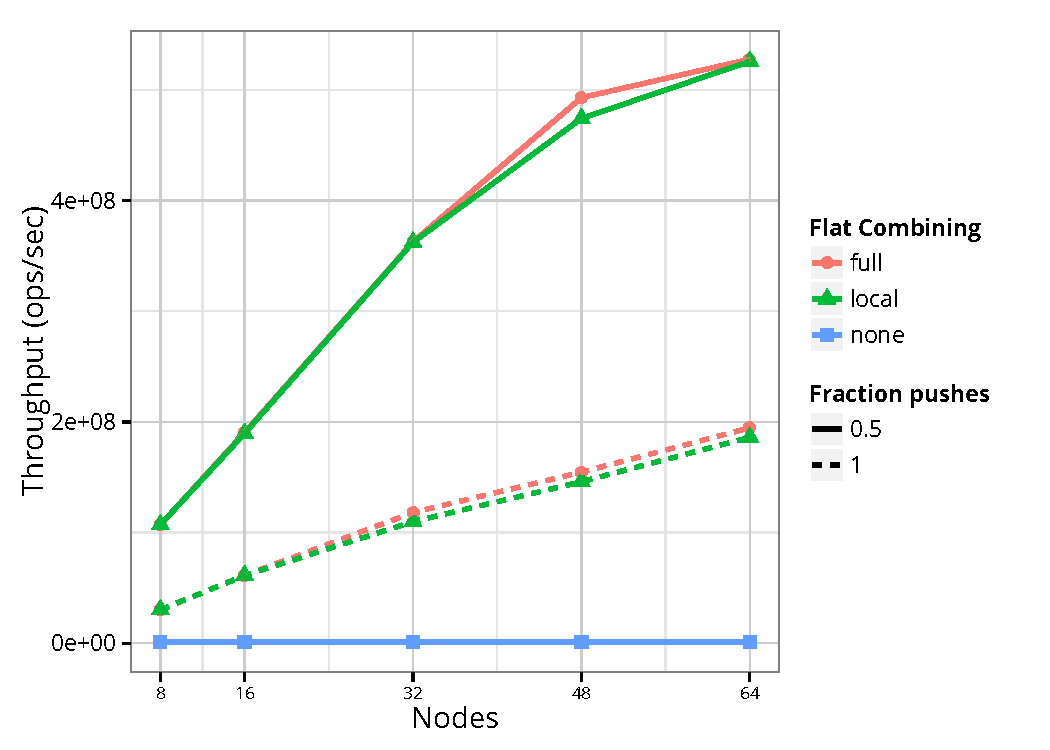
\includegraphics[width=\textwidth]{data/plots/stack_perf.pdf}
  \caption{Stack performance.}
  \label{fig:stack}
  \end{subfigure}%
  \hspace{0.05\textwidth}
  % ~ %add desired spacing between images, e. g. ~, \quad, \qquad etc.
  %(or a blank line to force the subfigure onto a new line)
  \begin{subfigure}[b]{0.45\textwidth}
  \centering
  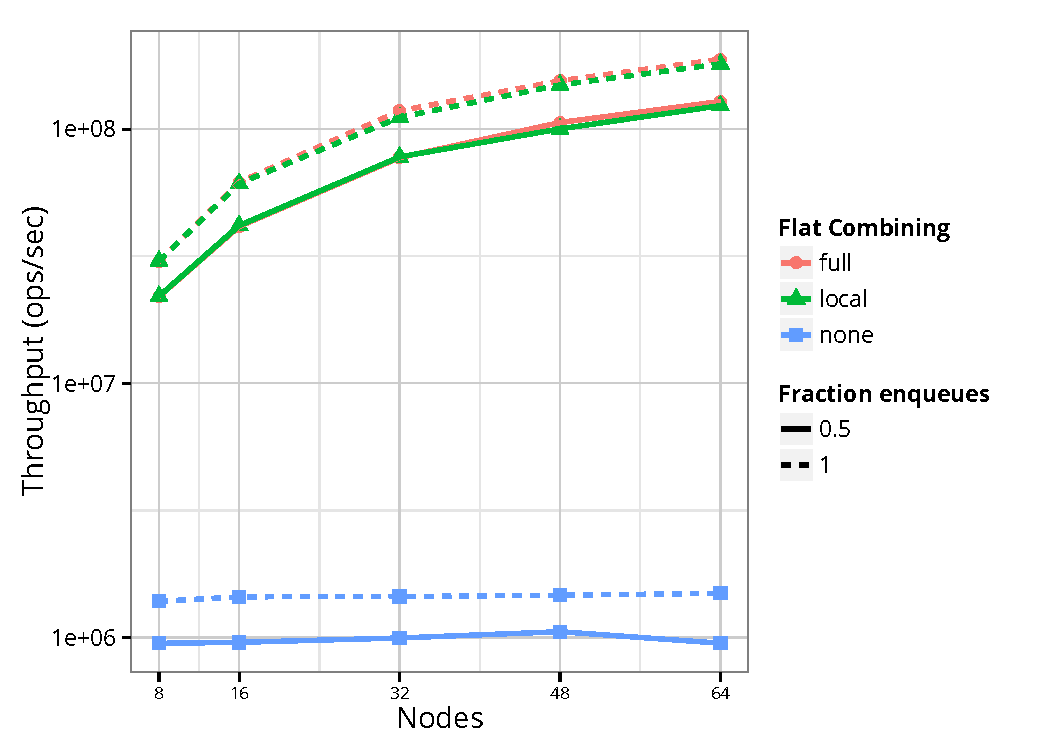
\includegraphics[width=\textwidth]{data/plots/queue_perf.pdf}
  \caption{Queue performance.}
  \label{fig:queue}
  \end{subfigure}
  
  \begin{subfigure}[b]{0.45\textwidth}
  \centering
  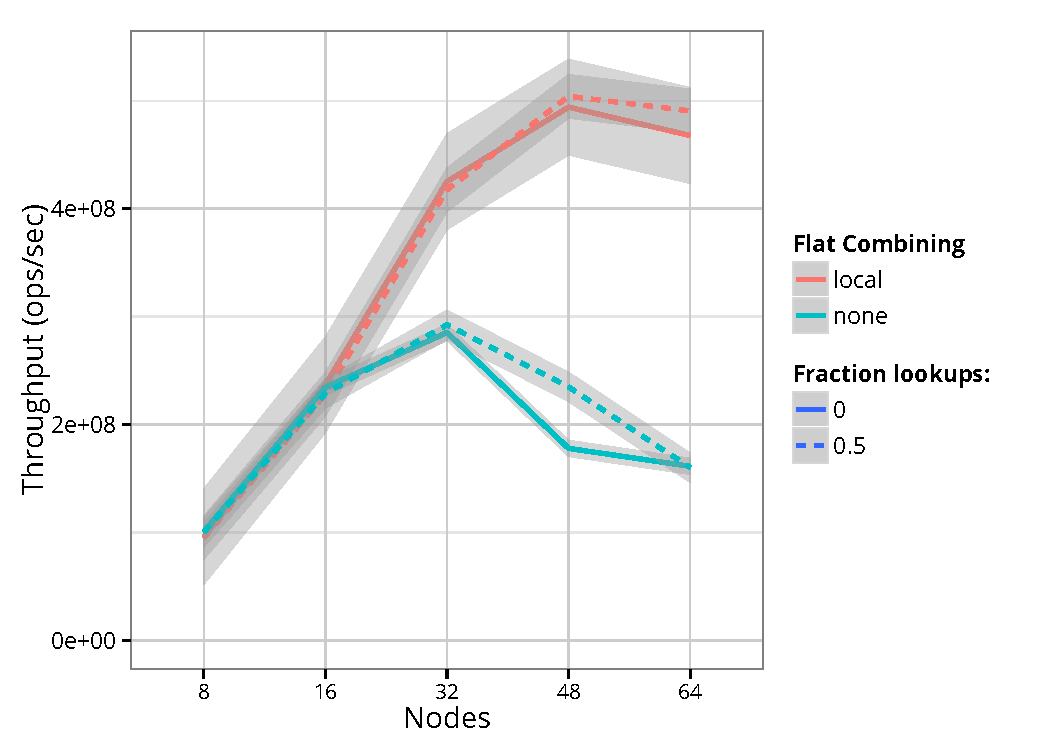
\includegraphics[width=\textwidth]{data/plots/hashset_perf.pdf}
  \caption{GlobalHashSet performance.}
  \label{fig:hashset}
  \end{subfigure}
  %
  \hspace{0.05\textwidth}
  %
  \begin{subfigure}[b]{0.45\textwidth}
  \centering
  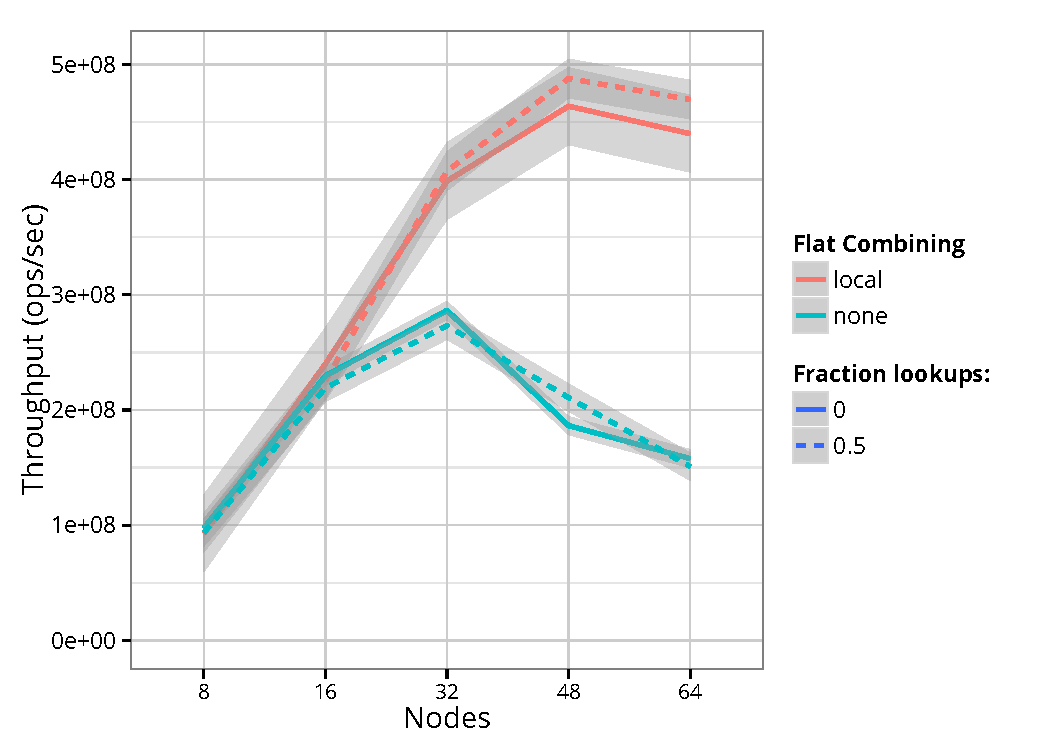
\includegraphics[width=\textwidth]{data/plots/hashmap_perf.pdf}
  \caption{GlobalHashMap performance.}
  \label{fig:hashmap}
  \end{subfigure}%
  %
  \caption{Raw performance of global data structures.
    \TODO{describe results.}
    \TODO{either all with error bars or none.}
  }\label{fig:datastructs}
\end{figure*}

\paragraph{Queue and Stack}
The GlobalQueue and GlobalStack have very similar implementations in terms of how they are synchronized. Both benefit greatly from flat combining. This is because only one round-trip message 

However, due to the nature of concurrent stacks, the stack is able to match up pushes and pops locally. This leads to performance on an even mix of pushes and pops far outstripping the case where all pushes are performed due to requiring vastly less communication.

